\section{Method}
\label{sec:method}

%% Method overview figure (one column). Graphic: figures/method.png
%% The three panels and their (a)/(b)/(c) labels are baked into the image itself,
%% so this file is a single \includegraphics rather than three stacked ones.
%%   (a) DINOv3 retrieval from the pool of reference touches, with cosine similarity bars
%%   (b) coarse alignment by local feature matching, homography, and warping
%%   (c) learning-based refinement of the initial transfer
\begin{figure}[t]
  \centering
  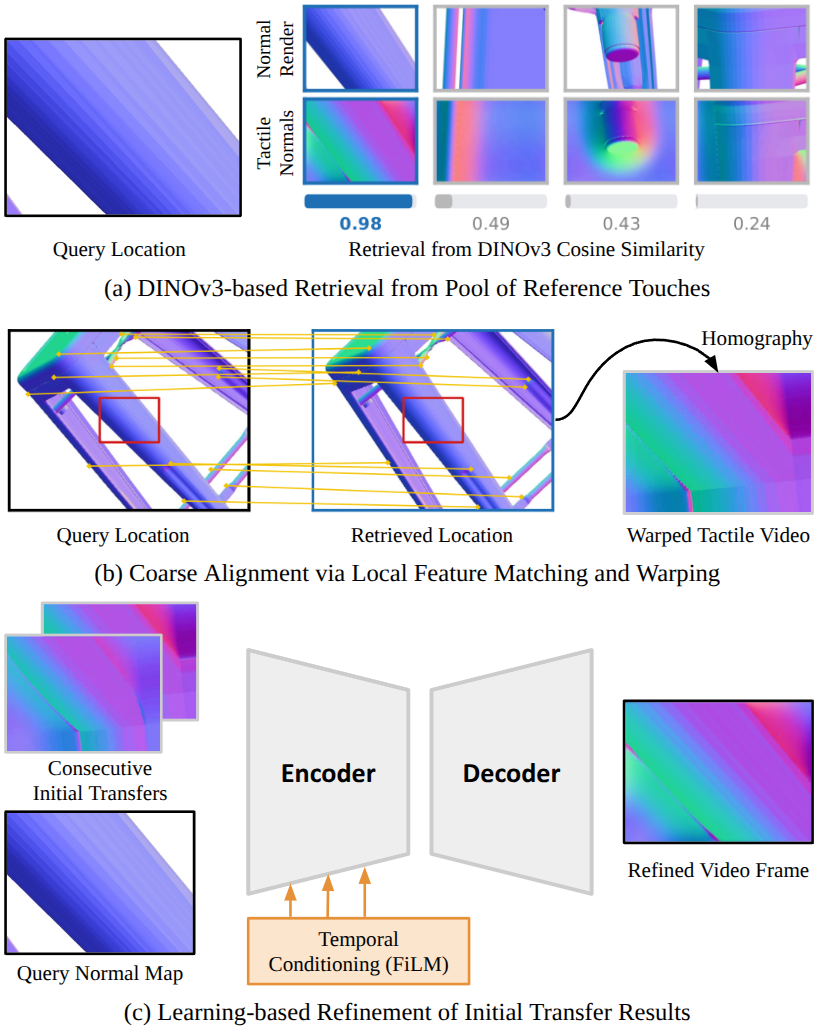
\includegraphics[width=\linewidth]{figures/method.png}
  \caption{\textbf{Method overview.} \emph{(a)} Every reference touch is stored alongside a
    surface normal render at its sensor pose, shown above its tactile normals. We encode the
    normal renders with a frozen DINOv3 encoder and score each reference against the query by
    cosine similarity, shown as the bar under each candidate, then keep the top-1 match
    (Sec.~\ref{sec:retrieval}). \emph{(b)} We match local features between the query normal render
    and the retrieved one, drawn here as yellow correspondences, and fit a homography to them. The
    homography warps the retrieved tactile video into the query frame to give the initial transfer
    (Sec.~\ref{sec:coarse}). The red box marks the patch the sensor itself covers inside the wider
    render. \emph{(c)} A lightweight encoder-decoder network refines the initial transfer. It
    receives a pair of consecutive initially transferred frames together with the query normal
    map, which tells it the surface geometry it is predicting for, and the normalized timestamp of
    the frame enters through feature-wise linear modulation (FiLM) so that the network knows where
    in the press it is (Sec.~\ref{sec:refine}).}
  \label{fig:method}
\end{figure}


\subsection{Overview}

As shown in Fig.~\ref{fig:method}, our method takes as input (i) a set of reference tactile normal
videos together with surface normal maps rendered at the same tactile sensor poses, and (ii) a set
of query tactile sensor poses at which we wish to predict tactile normal videos. We render normal
maps at the query poses as well, and use them as the geometric context for prediction.

Formally, let $\mathcal{R} = \{ (V_i, N_i) \}_{i=1}^{N}$ be the reference set, where
$V_i = (V_i^1, \dots, V_i^T)$ is a tactile normal video of $T$ frames and $N_i$ is the normal
map rendered at the pose of touch $i$. Given a query normal map $N_q$, our goal is to produce a
predicted video $\hat{V}_q$.

Obtaining the normal renderings does not require a mesh of the object at deployment time. In
practice one can (i) obtain a depth map from a commodity sensor such as a stereo camera,
(ii) take spatial gradients of the depth map to get a normal map in the camera frame, and
(iii) project those normals into the tactile sensor frame, using the relative pose between the
sensor and the camera. That relative pose is available either from forward kinematics, when both
are mounted on a robot, or from fiducial markers such as an ArUco tag attached to the back of the
sensor.

We then take a coarse-to-fine approach with three steps: retrieve the most promising reference
touch using DINOv3 features (Sec.~\ref{sec:retrieval}); coarsely align the two normal maps to
obtain an affine map that gives an initial transfer of the reference tactile video
(Sec.~\ref{sec:coarse}); and refine that initial transfer with a neural network
(Sec.~\ref{sec:refine}).

\subsection{Retrieval}
\label{sec:retrieval}

A reference touch is useful only if the surface it was taken on resembles the surface at the
query pose. We measure this resemblance in the space of a self-supervised visual descriptor.
Concretely, we render normal maps over a field of view larger than the sensor footprint --- four
times the sensor's extent by default --- so that the descriptor sees the surrounding surface
context and not just the small contact patch, and we extract the class-token feature of a
pre-trained DINOv3 encoder~\cite{dinov3}:
\begin{equation}
  f_i \;=\; \frac{\phi(N_i)}{\lVert \phi(N_i) \rVert_2},
  \qquad
  f_q \;=\; \frac{\phi(N_q)}{\lVert \phi(N_q) \rVert_2},
\end{equation}
where $\phi(\cdot)$ denotes the encoder. The retrieved reference is the one whose feature is most
similar in the cosine sense,
\begin{equation}
  i^{*} \;=\; \arg\max_{i \in \{1,\dots,N\}} \; f_i^{\top} f_q .
  \label{eq:retrieval}
\end{equation}
We use the top-1 result throughout. Because the descriptor is frozen and the features of the
reference set can be computed once and cached, retrieval reduces to a single matrix--vector
product at query time.

\subsection{Coarse Alignment}
\label{sec:coarse}

Retrieval tells us \emph{which} reference to use; alignment tells us \emph{how} to place it. Using
the top-1 retrieval $N_{i^{*}}$, we run a local feature matcher --- SuperPoint
keypoints~\cite{superpoint} matched by SuperGlue~\cite{superglue} --- between $N_{i^{*}}$ and
$N_q$, obtaining a set of $K$ two-dimensional pixel correspondences
$\{(\mathbf{p}_k, \mathbf{q}_k)\}_{k=1}^{K}$. From these we estimate an affine map
$\mathbf{A} \in \mathbb{R}^{2\times 3}$ under RANSAC~\cite{ransac}:
\begin{equation}
  \mathbf{A} \;=\; \arg\min_{\mathbf{A}} \sum_{k=1}^{K}
  \rho\!\left( \bigl\lVert \mathbf{A}\,\tilde{\mathbf{p}}_k - \mathbf{q}_k \bigr\rVert_2 \right),
  \label{eq:affine}
\end{equation}
where $\tilde{\mathbf{p}}_k$ is $\mathbf{p}_k$ in homogeneous coordinates and $\rho$ is the
RANSAC inlier--outlier cost.

We estimate $\mathbf{A}$ in two decomposed parts, because the two parts are best measured at
different fields of view. Matching over the wide, $4\times$ field of view gives many more
keypoints and therefore a far more stable estimate of the linear part (rotation, scale, shear);
but that estimate is expressed in wide-field pixels, and rescaling it down to the narrow field of
view that the tactile video actually covers amplifies any error in its translation component. We
therefore first solve Eq.~\ref{eq:affine} at the matching scale, rescale the result to video
resolution, and strip its translation so that the remaining linear map $\mathbf{A}_0$ fixes the
image centre. We then warp the reference normal map by $\mathbf{A}_0$ and re-match against the
query at video scale; since the linear part is already removed, the residual displacement is a
pure translation, and we take its component-wise median over the matches,
\begin{equation}
  \mathbf{t} \;=\; \operatorname{median}_{k} \bigl( \mathbf{q}'_k - \mathbf{p}'_k \bigr),
\end{equation}
with $\{(\mathbf{p}'_k, \mathbf{q}'_k)\}$ the matches found after warping. The final affine map is
$\mathbf{A} = [\,\mathbf{A}_0 \mid \mathbf{t}\,]$.

Applying $\mathbf{A}$ to every frame of the retrieved reference video gives the initial transfer
\begin{equation}
  W^{t} \;=\; \mathcal{W}\bigl( V_{i^{*}}^{t}; \, \mathbf{A} \bigr),
  \qquad t = 1, \dots, T,
  \label{eq:warp}
\end{equation}
where $\mathcal{W}$ denotes image warping. Note that a \emph{single} geometric transform is shared
by all frames: the sensor pose does not move relative to the surface during a press, so what
changes across the video is the gel deformation, not the alignment.

\subsection{Learning-based Refinement}
\label{sec:refine}

The initial transfer is geometrically plausible but physically naive. It carries whatever gel
dynamics the reference press happened to exhibit, it inherits any residual misalignment left by
Eq.~\ref{eq:affine}, and it knows nothing about the surface geometry at the query pose beyond what
survived the warp. Our final step corrects all three with a neural network. Since we target
prediction fast enough for AR/VR and robotics, we deliberately balance refinement accuracy against
efficiency.

\paragraph{Architecture.}
Our refinement network is based on ReBotNet~\cite{rebotnet}, a lightweight architecture for video
enhancement. ReBotNet processes a pair of consecutive frames through two branches --- a
ConvNeXt-style spatio-temporal branch and a per-frame token branch --- and merges them in a shared
decoder, with a global residual connection that adds the current input frame back to the
prediction. It was originally designed to remove blur and compression artifacts from natural
video, so we adapt it in two ways.

\emph{Normal map concatenation.} We concatenate the query normal render $N_q$ to the input as
three additional aligned channels, broadcast across both frames of the pair. This makes the
network aware of the rough surface geometry at the query location, which is exactly the
information the warped reference cannot supply.

\emph{Temporal conditioning with FiLM.} The normal map is static --- it is rendered once at the
query pose and does not change over the press --- so on its own it gives the network no sense of
where in the press it currently is. We therefore inject the frame's normalized timestamp
$\tau_t = (t-1)/(T-1) \in [0,1]$, which runs from no contact through deepest press to take-off.
Following the standard diffusion-model recipe, a fixed sinusoidal embedding of $\tau_t$ is passed
through a small multi-layer perceptron and mapped to a per-stage scale and shift, applied as
feature-wise linear modulation (FiLM):
\begin{equation}
  \mathrm{FiLM}(\mathbf{h}_s; \tau_t) \;=\;
  \bigl(1 + \gamma_s(\tau_t)\bigr) \odot \mathbf{h}_s + \beta_s(\tau_t),
\end{equation}
where $\mathbf{h}_s$ are the features at stage $s$. The heads producing $\gamma_s$ and $\beta_s$
are zero-initialized, so the module starts as an exact identity and departs from it only as
training justifies.

Writing the refinement network as $\mathcal{F}$, the prediction for frame $t$ is
\begin{equation}
  \hat{V}_q^{\,t} \;=\; \mathcal{F}\bigl( [\,W^{t-1}, W^{t}\,] \oplus N_q ; \; \tau_t \bigr),
  \label{eq:refine}
\end{equation}
with $\oplus$ denoting channel concatenation and $W^{0} := W^{1}$ for the first frame.

\paragraph{Training loss.}
We supervise with a Charbonnier loss, a smooth approximation to the $\ell_1$ distance that is less
sensitive to outliers than a squared error,
\begin{equation}
  \mathcal{L}_{\mathrm{ch}} \;=\;
  \frac{1}{|\Omega|}\sum_{x \in \Omega}
  \sqrt{\bigl(\hat{V}_q^{\,t}(x) - V_q^{t}(x)\bigr)^2 + \epsilon^2},
\end{equation}
evaluated on the region $\Omega$ where the ground-truth query frame differs from the warped input,
i.e.\ the part of the frame the network is actually being asked to change. \new{We add a small
penalty on the magnitude of the correction the network applies,
\begin{equation}
  \mathcal{L} \;=\; \mathcal{L}_{\mathrm{ch}}
  \;+\; \lambda \, \bigl\lVert \hat{V}_q^{\,t} - W^{t} \bigr\rVert_1 ,
\end{equation}
which discourages large edits unless the data justifies them and keeps the network anchored to the
geometrically grounded initial transfer.}
